\section{Door task}
	\label{sub:door}

\subsection{Outline of the door task}
\label{sub:OutlineDoor}
%
At the DRC Finals, the door task was especially important because without passing through it,
the robot wouldn't be able to perform the five remaining tasks
(valve, wall, surprise, debris or terrain, and stairs).
We can divide its execution into the following phases:
%
\begin{enumerate}
	\item Walking to the front of the door.
	\item Grasping the door lever.
	\item Turning the lever and opening the door.
	\item Walking through the door.
\end{enumerate}
%

%In the DRC Finals, it was announced that the door will be 
%
%\begin{itemize}
%\item push open style,
%\item with lever type door lever, and
%\item without door closer.
%\end{itemize}

At the end of the second phase, the robot ends up in a standing configuration with a hand grasping
the door lever.
In our approach, we determine a specific standing stance and a wrist pose with respect to 
the door lever as shown in \figurename~\ref{fig:door_approaching_config}.

Let us call this the {\it open-door pose}.
This is important since it connects the free space motion and the constrained motion by
the door mechanism. 
Phase 3) always starts from this configuration and is followed by phase 4).
Since the open-door pose determines the initial state of the robot and the door, 
we can use a pre-programmed sequence for operating the door and passing through it.
%In this way, the remaining phases 3) and 4) start from the same configuration;
%Even if we face variations of the door's geometry, they can be handled by means of a minimum modifications.

\begin{figure}[t]
  \centering
  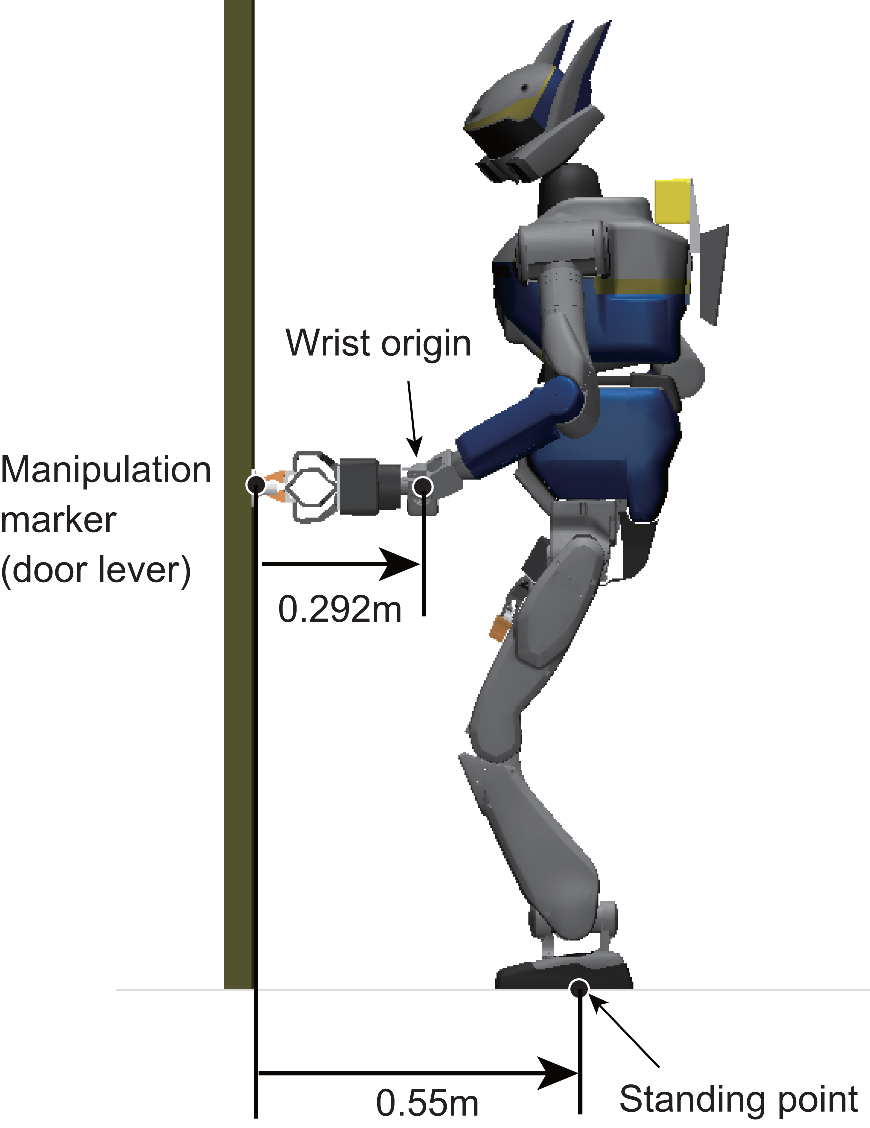
\includegraphics[width = 5.5cm]{img/door_approaching_config}
  \caption{Open-door pose}
  \label{fig:door_approaching_config}
\end{figure}

%From Step1 to Step2, we control our robot to realize the door approaching pose.
%To realize a reliable door passing, we pre-determined
%a robot pose grasping the door lever.
%Let us call it as {\it door approaching pose} which specifies the
%wrist point and the standing point with respect to the door lever

%The door lever operation (Step3) and the door passing through (Step4) always start
%from this fixed configuration. This means we can use a programmed sequence or its minimum
%modification at the door task.  

In the following subsections, we explain phases 1), 2), and 3); that is,
the way to control the robot to achieve the open-door pose and to manipulate the door.

Phase 4) could be easily implemented at the DRC Finals in the absence of door-closers 
and given that the door was inclined 2.6 deg away from the vertical.
Once the door had been opened wide enough, it opened completely by gravity.
This helped the robots to walk through the door without colliding with the door panel.
In the DRC Trials 2013, it was more difficult since some of the doors had spring closers.

\subsection{Walking to the front of the door}
%
To navigate the robot to the pose specified in \figurename~\ref{fig:door_approaching_config},
we used the point cloud data measured by the LRF. 
Then, we took a sequence of steps to identify the door orientation and the position of the
door lever as illustrated in \figurename~\ref{fig:door_manip_markers}.

First, the operator specifies a point on the left edge of the door panel
(\figurename~\ref{fig:door_manipulation_markers_a} the `x' mark pointed by the arrow).
By applying the least square method to the portion of the point cloud located at the right of
the specified point, we can calculate the orientation of the door panel.
The result is shown by the {\it door marker}, a gray rectangle in
\figurename~\ref{fig:door_manipulation_markers_b}.
It covers a part of the door panel and we can interactively manipulate it on the point cloud GUI.
By adjusting the door marker, we can mask the points of the door panel and extract the points of
the door lever as shown in \figurename~\ref{fig:door_manipulation_markers_c}.
In this way, we can confidently mark the rotation center of the lever (pointed by the arrow).
\figurename~\ref{fig:door_manipulation_markers_d} shows the manipulation marker for the door lever
placed on the point cloud.
Its position and orientation are used to navigate the robot to the standing point of the open-door pose.
As an alternative method, it might be possible to use the model alignment function of the PCL library
as in Section~\ref{sub:DetectionSocketPlug}.
However, it is difficult to use the conventional model fitting since the point cloud corresponding to
the door lever contains only 10 to 20 points due to our LRF resolution. 
For this reason, we chose the above method relying on human perception.

\begin{figure}[t]
	\centering
	\subfloat[Set an attention point on the point cloud]
		{\label{fig:door_manipulation_markers_a} 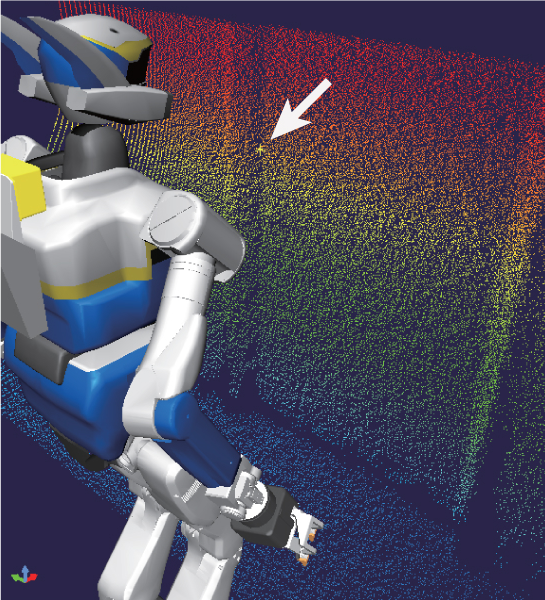
\includegraphics[width = 3.25cm]{img/door_manipulation_markers_a}}
	\quad
	\subfloat[Manipulation marker for the door panel]
		{\label{fig:door_manipulation_markers_b} 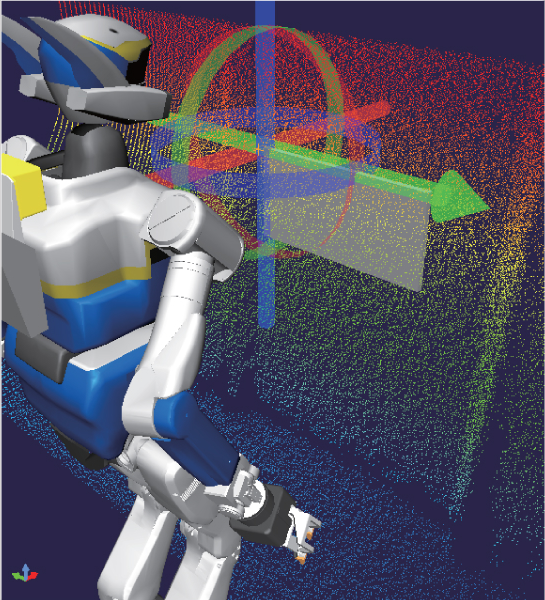
\includegraphics[width = 3.25cm]{img/door_manipulation_markers_b}}
	\\
	\subfloat[Set the second attention point on the lever axis]
		{\label{fig:door_manipulation_markers_c} 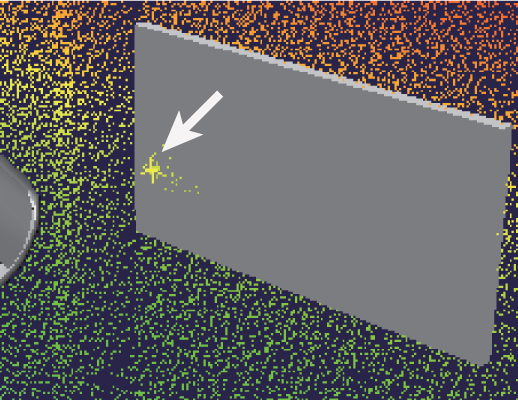
\includegraphics[width = 3.25cm]{img/door_manipulation_markers_c}}
	\quad
	\subfloat[Manipulation marker for the lever]
		{\label{fig:door_manipulation_markers_d} 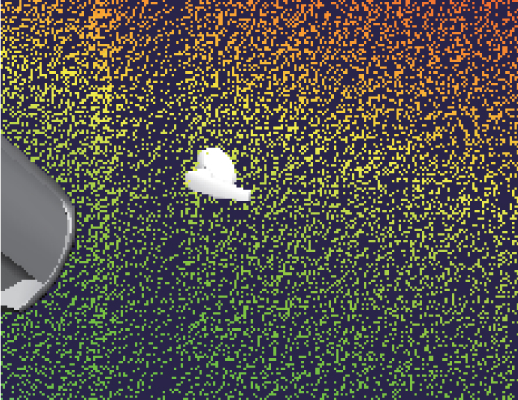
\includegraphics[width = 3.25cm]{img/door_manipulation_markers_d}}
	\\
	\caption{Detection of the door lever in the control window}
	\label{fig:door_manip_markers}
\end{figure}

\subsection{Grasping the door lever}
\label{sub:GraspLever}
%
One might expect that the robot can grasp the door lever autonomously from the standing point.
However, it is not appropriate since the hand position is not accurate enough due to the 
LRF measurement noise, calibration error, and foot slip while walking.

Instead of grasping the door lever directly, we move the robot hand to an {\it approach point},
which is placed at a certain distance (0.13 m) from the target, then adjust it
by using the camera image to guarantee a secure grasp.

%Although the robot is standing pararell to the door, its position is not accurate enough to 
%grasp the door lever due to the calibration error and the LRF measurement noise. 

%at a good place to grasp the door levre
%In free space, there always exists a few centimeter error with respect 
%to the LRF measurement, while a robot hand requires a few millimeter accuracy for reliable touch
%or grasp.   From this reason, our robot cannot directly grasp a target sensed by LRF. 

%Now the robot is standing at a good place to grasp the door lever.
%Instead of grasping the door lever directly, we move the robot hand to an {\it approach point},
%which is placed at a certain distance (0.13m) from the lever. 
%This is because the hand position may not be accurate enough due to the LRF measurement noise,
%calibration error, and slip occurring while walking.

\figurename~\ref{fig:approach_door_lever_a} shows the robot at the standing point and its hand at the
approach point (right window) in Choreonoid simulator.
The left window shows the simulated view of the left hand camera.
From the hand camera image, we can see that the hand is not correctly aligned 
to grasp the lever (the hand is located too at the left and too low with respect to the lever). 
Notice that during the real robot control, only the camera view is available. 

The operator can adjust the hand position by using the GUI buttons: 
{\it Left}, {\it Right}, {\it Down}, and {\it Up} on the task sequencer panel at the bottom left.
In this case, the operator can adjust the hand position by hitting {\it Right} and {\it Up} button
several times.
\figurename~\ref{fig:approach_door_lever_b} shows the adjusted hand position to grasp the lever.
By hitting the button 'OK', the robot moves the hand forward until it touches the door surface
(we specified a threshold of 5 N to detect the contact).
Then the robot retracts the hand by a specified distance (0.01 m) to avoid the finger tips to scuff
the door surface.

\figurename~\ref{fig:approach_door_lever_c} shows the final state getting a good grasp of the door lever.
From the hand camera image, we can be convinced that the robot is actually at the open-door pose.
This means that the rotation center of the door lever is at the planned position with respect to the 
current wrist position obtained from the joint encoders, posture sensors and the dead-reckoning data.
The point cloud data is not used from this moment, since it is not reliable anymore.

%For example, the rotation center of the lever is determined using the hand position calculated from
%the internal sensors (joint encoders and posture sensors). 
%
\begin{figure}[t]
	\centering
	\subfloat[Initial state for door lever approaching]
		{\label{fig:approach_door_lever_a} 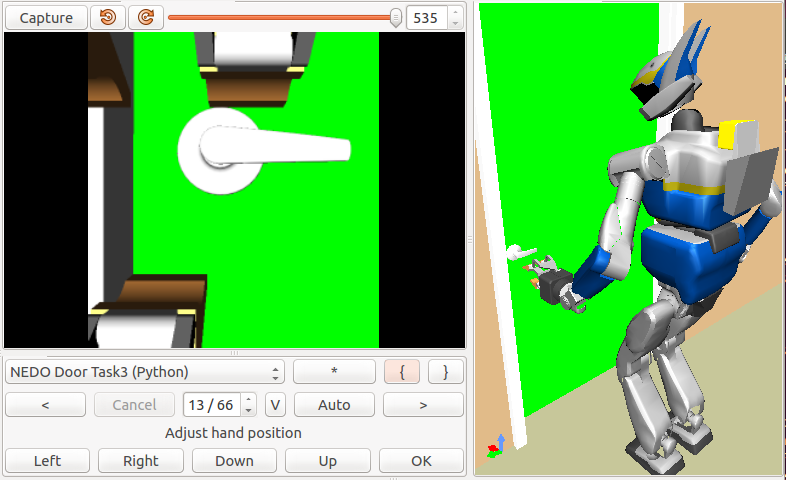
\includegraphics[height = 3.1cm]{img/approach_door_lever_a}}
	\\
	\subfloat[Hand position was adjusted]
		{\label{fig:approach_door_lever_b} 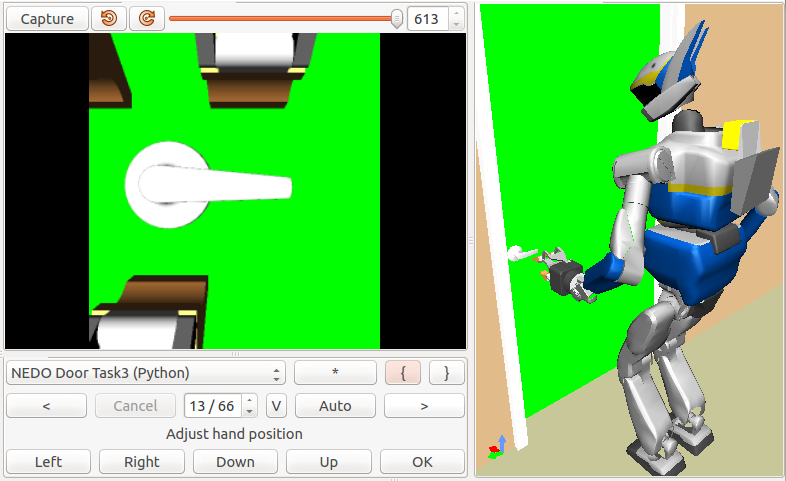
\includegraphics[height = 3.1cm]{img/approach_door_lever_b}}
	\\
	\subfloat[The door lever grasped]
		{\label{fig:approach_door_lever_c} 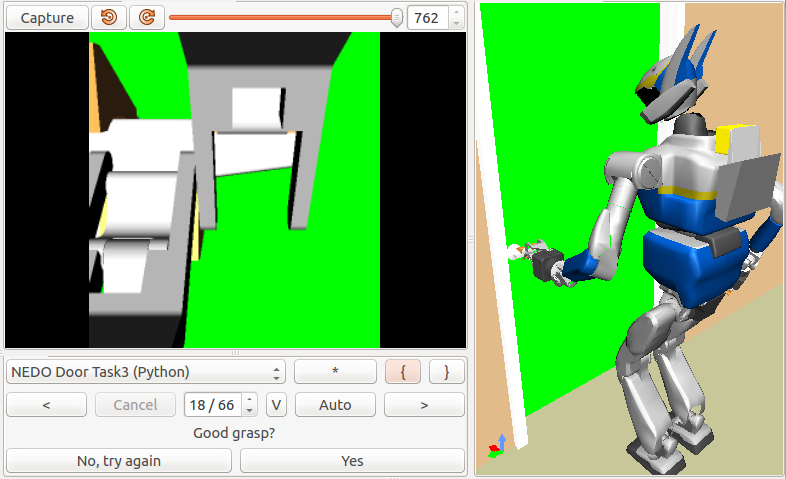
\includegraphics[height = 3.1cm]{img/approach_door_lever_c}}
	\\
	\caption{Approach for grasping the door lever}
	\label{fig:door_lever_grasp}
\end{figure}

%\begin{figure}[t]
%  \centering
%  \includegraphics[width = 7.5cm]{img/open_the_door}
%  \caption{Door opening}
%  \label{fig:door_opening}
%\end{figure}

\subsection{Turning the lever and opening the door}
\label{sub:TurningLever}

Having the lever grasped with left hand, the door can be opened by using the following sequence:
%
\begin{itemize}
\item[{\bf step1}] Turn the lever 30 deg around the rotation axis.
\item[{\bf step2}] Push forward the lever 0.1 m and stop if the reaction exceeds 25 N.
\item[{\bf step3}] Check the camera image; if the door is opened go to step5.
\item[{\bf step4}] Turn the lever 7 deg more and go to step3.
\item[{\bf step5}] Turn back the lever to its neutral orientation.
\item[{\bf step6}] Open the hand and release the door. 
\end{itemize}
%
The hard-coded parameters like the rotation of 30 deg, the reaction force limit of 25 N, etc.
were determined based on the experiments with a door mock-up that we prepared.

\subsection{Result at the DRC Finals}
%
In the DRC Finals 2015, HRP-2Kai cleared the door task at the rehearsal on June 4 and at the challenge on June 6.
Figure \ref{fig:drc_door_aist_day2} shows the robot (a) while scanning with the LRF to
obtain a point cloud, (b) walking to the open-door pose, (c) grasping the door lever,
and (d) opening the door successfully.
The robot spent 5 minutes and 21 seconds from the LRF scan to fully pass the door.
%
\begin{figure}[t]
	\centering
	\subfloat[LRF measurement 17:57:09 06/06/2015 UTC]
		{\label{fig:drc_door_aist_day2_a} 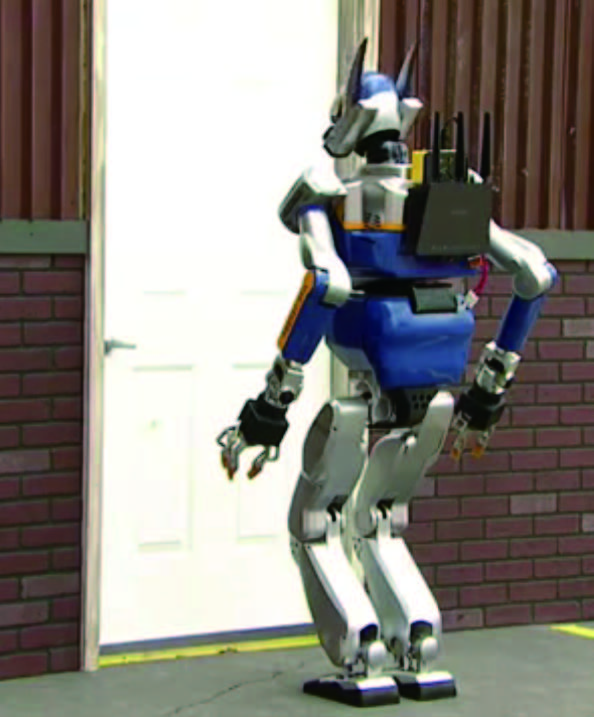
\includegraphics[height = 3cm]{img/drc_door_aist_day2_a}}
	\quad
	\subfloat[Walk to open-door pose 17:57:50 06/06/2015 UTC]
		{\label{fig:drc_door_aist_day2_b} 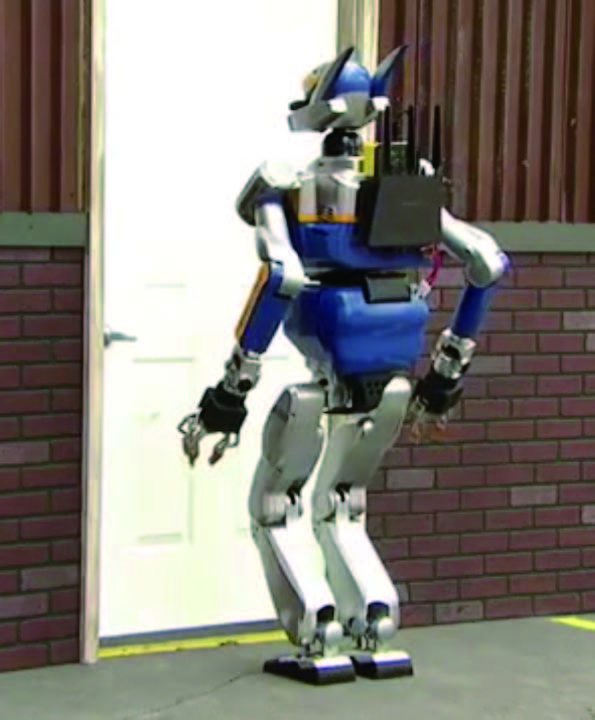
\includegraphics[height = 3cm]{img/drc_door_aist_day2_b}}
	\\
	\subfloat[Robot at open-door pose 17:57:09 06/06/2015 UTC]
		{\label{fig:drc_door_aist_day2_c} 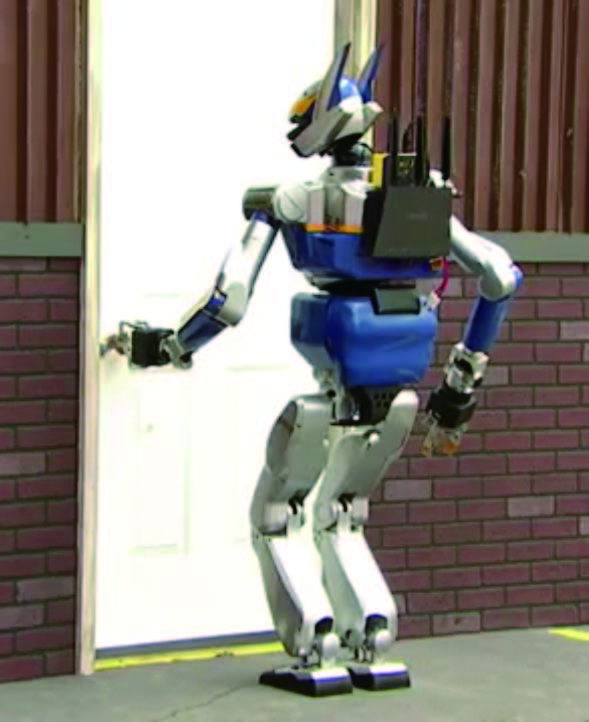
\includegraphics[height = 3cm]{img/drc_door_aist_day2_c}}
	\quad
	\subfloat[The door was opened 17:59:57 06/06/2015 UTC]
		{\label{fig:drc_door_aist_day2_d} 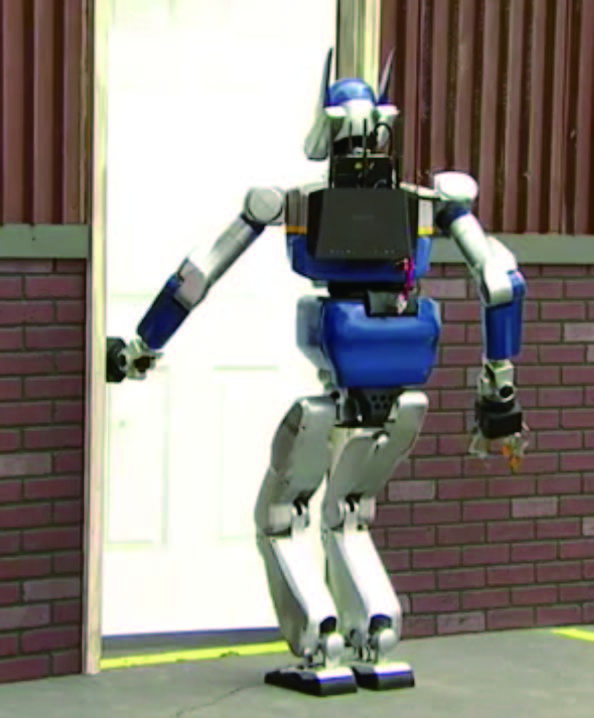
\includegraphics[height = 3cm]{img/drc_door_aist_day2_d}}
	\\
	\caption{Door task at DRC Finals on June 6~\cite{DARPA}}
	\label{fig:drc_door_aist_day2}
\end{figure}

At the challenge on June 5, HRP-2Kai couldn't open the door at step3 (Section~\ref{sub:TurningLever})
and turned the lever 7 deg more (step4).
After that, the lever had slipped out from the hand due to a loose of grasp and the strong spring.
Thus, we decided to retry the phase 3) (Section \ref{sub:OutlineDoor}), which required a whole body
motion planning to go again to the open-door pose.
%requiring a second attempt to grasp it again, which was done by manual teleoperation.
When we sent the planned trajectory to the robot, we experienced a crash on the feedback control
which might have been caused by a Not-A-Number (NAN) generated by our trajectory planner, and the
robot fell down (\figurename~\ref{fig:drc_door_aist_day1}).
Since the computer stopped working and the hardware had been damaged, we had to abort the
challenge for that day. 
%
\begin{figure}[t]
  \centering
  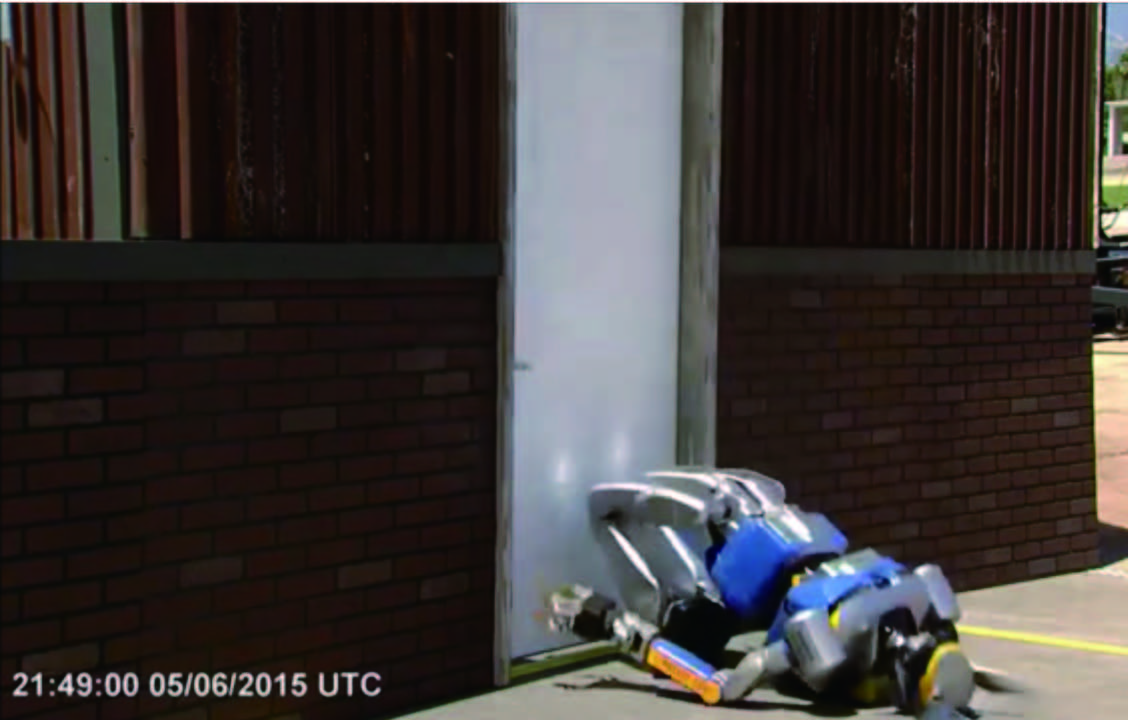
\includegraphics[width = 4.5cm]{img/drc_door_aist_day1}
  \caption{Control system crash at DRC Finals on June 5~\cite{DARPA}}
  \label{fig:drc_door_aist_day1}
\end{figure}

The robot failed to operate the lever because the doors of the DRC Finals had different
latch properties, as shown in Table~\ref{tbl:door_latch}.
We had hard-coded the latch rotation angle at step1 with 30 deg.
It worked at the rehearsal but it did not work on June 5.
On June 6, we changed the angle of step1 from 30 deg to 50 deg and it worked.
Of course, such implementation is not good for the actual disaster response robots.
%
\begin{table}[b]
\caption{Door latch properties at DRC finals} \label{tbl:door_latch}
\begin{tabular}{lclc}
\hline
Course & Latch release angle & Date & Door task result  \\ 
\hline
Green & 30 deg & June 4 (rehearsal) & Success  \\
Yellow & 70 deg & June 5 (day 1) & Fail \\
Blue &  50 deg & June 6 (day 2)  & Success \\
\hline
\end{tabular}
\end{table}

